\chapter{Trabalhos Relacionados}
\label{ch:trabalhosRelacionados}

Existem diversas plataformas que utilizam a LMS e gamificação para ensinar algum conteúdo a um grupo. Muitas dessas páginas Webs contém algumas semelhanças com a GameInfor. Contudo, mesmo sabendo que todas essas plataformas  têm como objetivo explicar uma temática através de uma série de etapas, elas possuem algumas importantes diferenças na sua proposta, essas diferenças podem definir o público alvo, o interesse do aluno nos tópicos passados e o custo benefício do uso de uma página específica.

Neste capítulo serão mostraremos algumas dessas plataformas, para cada uma delas apresentaremos as suas funcionalidades, o seu público alvo, seus pontos positivos e negativos. As plataformas que vamos abordar são: Engage, Apta, Moodle, Kaptiva e Dokeos.

\section{Engage}

A engage é uma plataforma de ensino que pode ser acessada através do link https://www.engage.bz, ela fornece ao usuário a possibilidade de criar uma série de cursos sobre os mais diversos conteúdos. Esta plataforma tem como público alvo as empresas que desejam fornecer aos seus funcionários cursos diversos. A ideia da mesma é que a empresas façam uso de seus recursos para passar os conhecimentos aos empregados.

Está é uma plataforma gamificada, ou seja, ela utiliza conceitos de jogos para tornar o conteúdo mais atraente aos funcionários que participarão do curso. Alguns dos conceitos utilizados são:

\begin{itemize}
\item Jogo de perguntas: nesses jogos são utilizadas animações para atrair visualmente o usuário, um relógio de pontos, nessa funcionalidade o usuário terá uma pontuação máxima para responder a pergunta, a medida que o tempo passar os pontos que serão recebidos caso a pergunta seja respondida de forma correta vai diminuindo.
\item Ranking: com essa funcionalidade o usuário pode competir amigavelmente com seus colegas de trabalho, verificando quem está obtendo a melhor pontuação no curso.
\item Conquistas pessoais: além de acompanhar o ranking geral de todos que estão fazendo o curso, a pessoa também pode acompanhar seu próprio andamento.
\item Avatar: o indivíduo pode também criar avatar escolhendo características como sexo, cor da pele, cabelo, olho, boca e nariz.
\end{itemize}

Resumindo, essa é uma boa plataforma, porém ela tem como desvantagem o fato de ser paga e ter um escopo de usuários limitada.

\begin{figure}[htp]
\begin{center}
  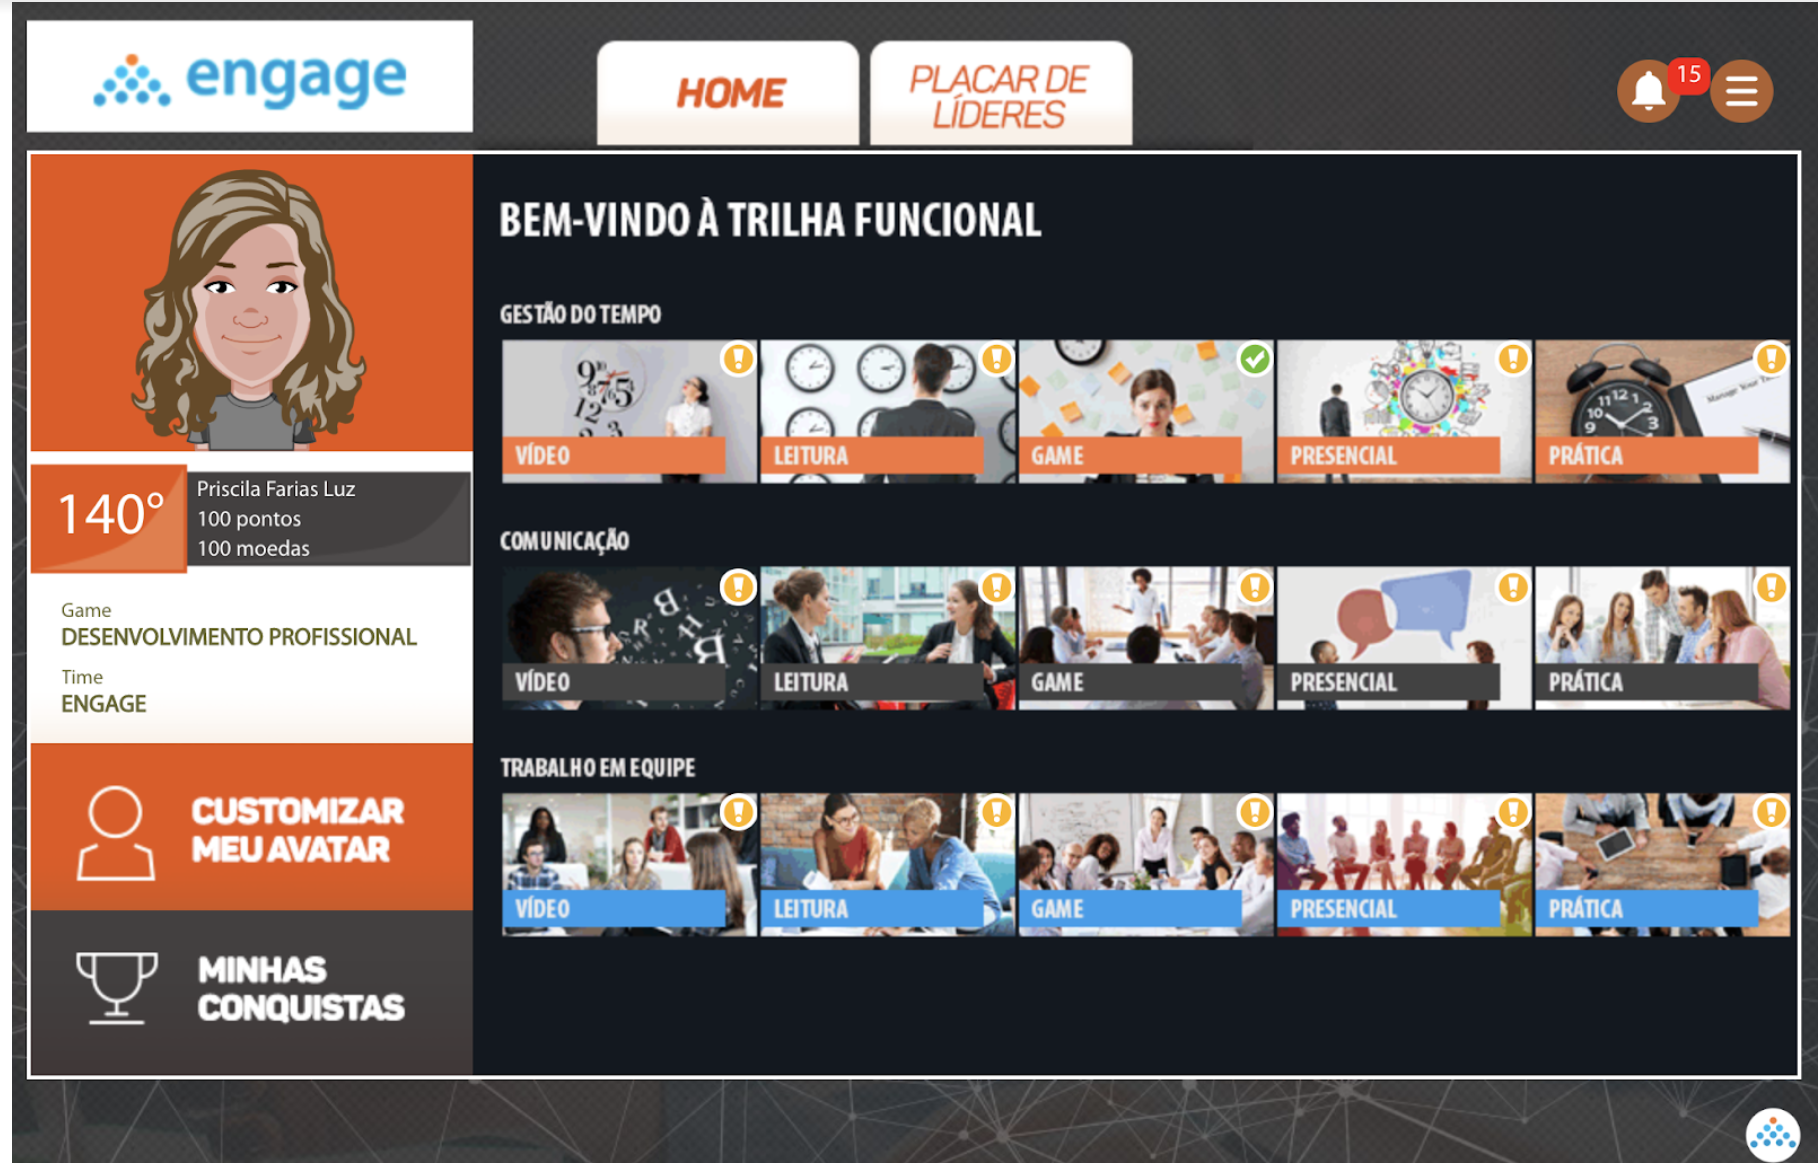
\includegraphics[width=15cm]{images/trabalhos-relacionados-img/img1-Engage.png}
  \caption{Exemplo da Plataforma Engage}
  \label{fig:exampleEngage}
\end{center}
\end{figure}


\section{Apta}

Ao acessar https://aptacursos.com.br  o usuário já encontrará a proposta do site que é "ser um ambiente de aprendizagem gamificado que promove informações inovadoras em áreas técnicas e profissionais, através de cursos onlines".

Nessa plataforma só tem permissão de criar novos cursos os proprietário criadores da mesma, porém um usuário pode requisitar a criação de um curso, para isso ele deve entrar em contato através do email ou telefone disponível na plataforma. Porém, é necessário destacar que essa é uma plataforma paga, ou seja, existe um custo associado à criação de um novo curso.

Como já foi dito, a Apta também utiliza alguns dos conceitos dos games na criação de seus cursos, a seguir serão enumerados alguns deles:

\begin{itemize}
\item A plataforma transforma cada curso é uma missão composta por uma série de desafios
\item Os desafios são de natureza diversa e podem incluir mini-jogos, quizzes, hipertextos, vídeos
\item A plataforma define metas a serem alcançadas pelos usuários do curso
\item Os alunos podem monitorar seu andamento através de ferramentas de avaliações
\end{itemize}

\begin{figure}[htp]
\begin{center}
  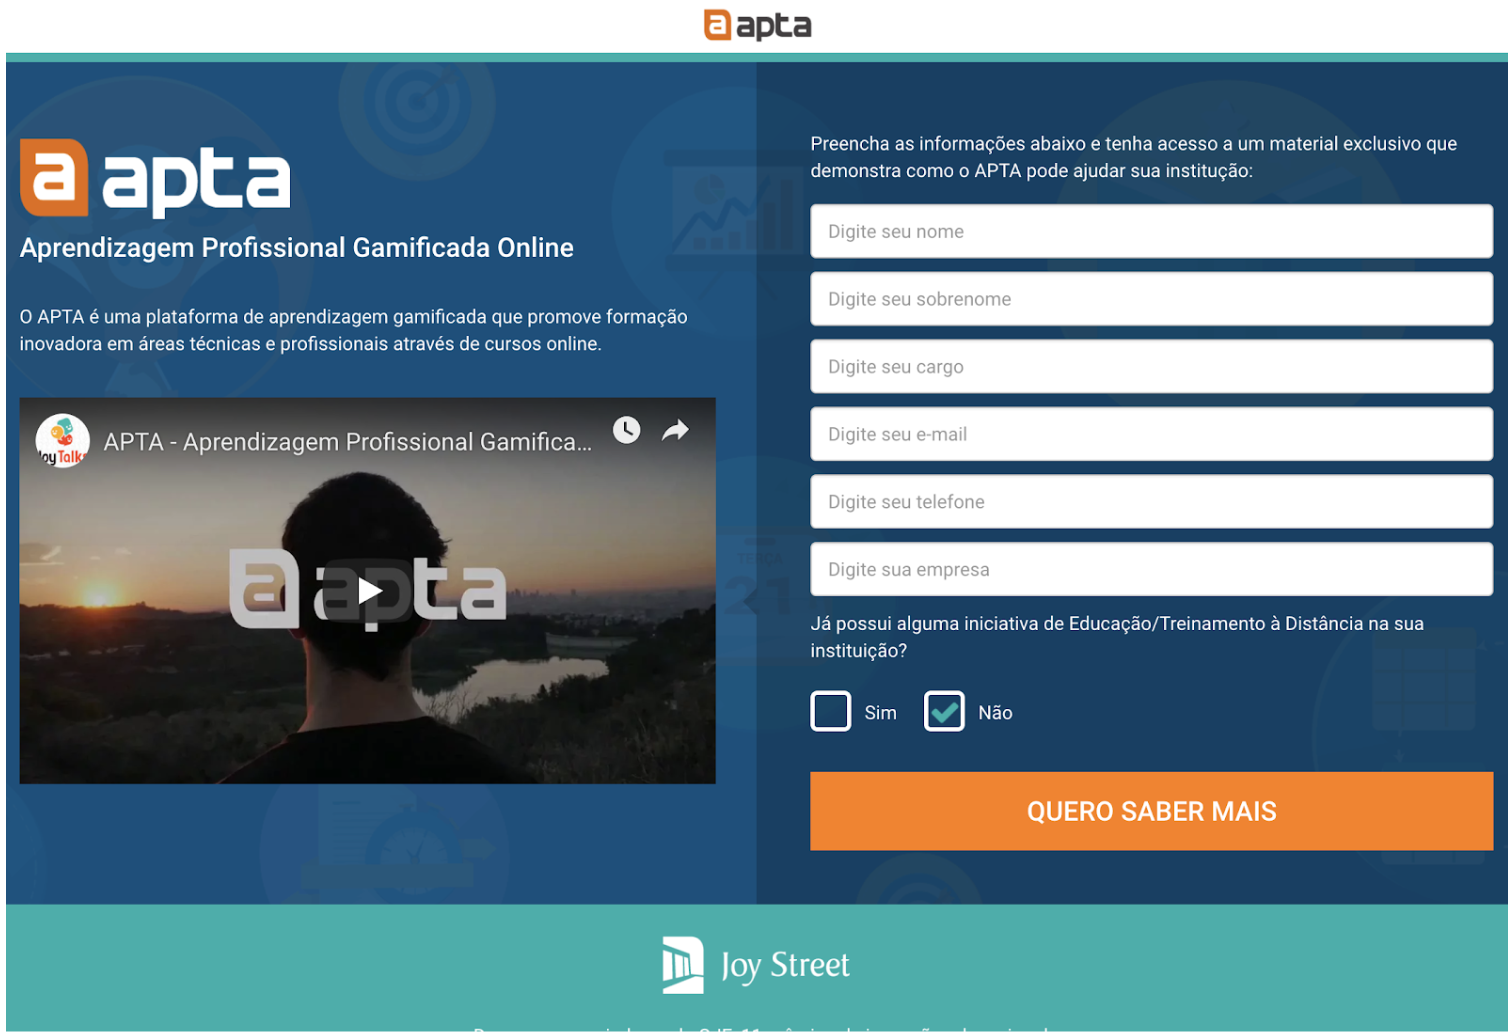
\includegraphics[width=12cm]{images/trabalhos-relacionados-img/img2-Apta.png}
  \caption{Exemplo da Plataforma Apta}
  \label{fig:exampleApta}
\end{center}
\end{figure}


\section{Moodle}

O moodle (Modular Object-Oriented Dynamic Learning Environment) é um software livre, que permite a criação de cursos, grupos de trabalho, páginas de disciplinas e comunidades. A primeira versão deste software foi disponibilizada em 2002 por seu criador Martin Dougiama, inicialmente ela foi criada para ser utilizada em faculdades, porém com o tempo ela invadiu outros ambiente como escolas e trabalho. Em questões de meses a plataforma ganhou o mundo e atualmente detém o título de ser a LMS mais popular que existe com 80 milhões de usuários em 222 territórios em todo o mundo. 

Algumas das funcionalidades existentes dentro dessa poderosa ferramenta são:

\begin{itemize}
\item Criações de cursos
\item Questionários
\item Avaliação dos professores
\item Criar comunidades em que os participantes possam se comunicar
\item Possibilidade do aluno de acompanhar suas próprias atividades
\end{itemize}

Como já foi mencionado, essa é uma poderosa ferramenta para ensino de conteúdo online, porém, um ponto negativo é que ela só permite ao professor criar cursos tradicionais, sem o uso de recursos visuais ou conceitos da gamificação.

\begin{figure}[htp]
\begin{center}
  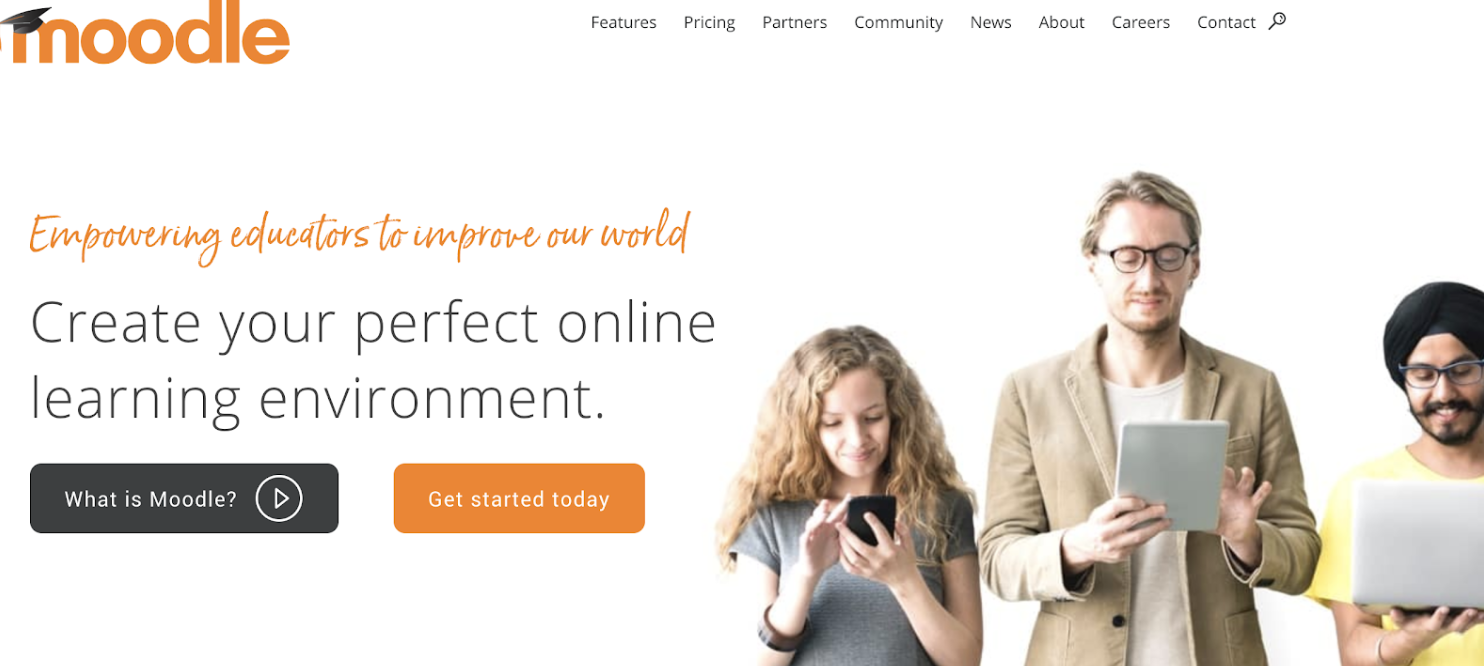
\includegraphics[width=10cm]{images/trabalhos-relacionados-img/img3-Moodle.png}
  \caption{Exemplo da Plataforma Moodle}
  \label{fig:exampleMoodle}
\end{center}
\end{figure}



\section{Kaptiva}

Mais uma plataforma de ensino que utiliza a gamificação nos seus cursos é kaptiva, esse ambiente de aprendizagem pode ser acessada através do link kaptiva.com.br.

Em sua página na Web ela demonstra ter como objetivo ser um "moodle gamificado". No tópico anterior já apresentamos a plataforma moodle e suas propostas, a diferencial da Kaptiva com relação ao moodle são basicamente três, a primeiro é o uso da gamificação feita por essa plataforma, algo que o moodle não se propõe a fazer, a segunda é ter como público alvo apenas empresas e por fim, temos a terceira que é o fato dessa plataforma ser paga diferente do moodle que como relatamos pode ser utilizado em diferentes ambiente de forma gratuita.

\begin{figure}[htp]
\begin{center}
  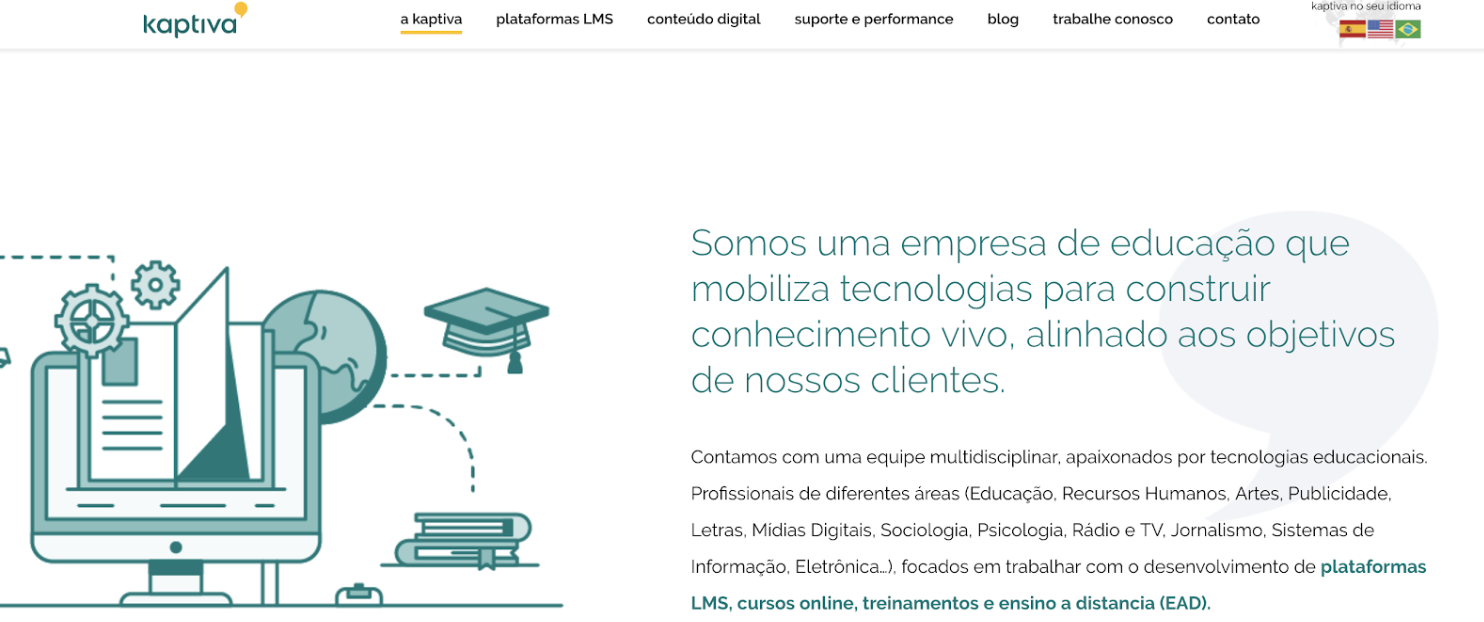
\includegraphics[width=15cm]{images/trabalhos-relacionados-img/img4-Kaptiva.png}
  \caption{Exemplo da Plataforma Kaptiva}
  \label{fig:exampleKaptiva}
\end{center}
\end{figure}

\section{Dokeos}

O Dokeos, assim como o moodle, é uma LMS que não utiliza a gamificação, nessa plataforma, os professores podem criar cursos onlines para disponibilizar a um grupo de alunos, após os alunos começarem a utilizar o professor tem a opção de acompanhar o andamento de cada participante.

Esse ambiente de aprendizagem pode ser acessada através do link www.dokeos.com, além disso é site multiplataforma e tem a desvantagem de ser paga.

\begin{figure}[htp]
\begin{center}
  
\includegraphics[width=15cm]{images/trabalhos-relacionados-img/img5-Dokeos.png}
  \caption{Exemplo da Plataforma Dokeos}
  \label{fig:exampleDokeos}
\end{center}
\end{figure}

